\section{Centro di Massa del Corpo Rigido e Simmetrie}
Il corpo rigido, in generale, è un sistema di punti materiali \textbf{continuo}. Pertanto, la definizione di centro di massa passa da una sommatoria discreta a un integrale esteso a tutto il volume del corpo:
\begin{equation}
    \vec{R}_{CM} = \frac{\int_{CR} \vec{r} \, dm(\vec{r})}{\int_{CR} dm(\vec{r})}
\end{equation}
dove l'integrale è limitato al volume occupato dal corpo rigido (CR).

È utile introdurre la \textbf{funzione densità di massa} volumetrica:
\begin{equation}
    \rho(\vec{r}) = \left. \frac{dm}{dV} \right|_{\vec{r}} \implies dm(\vec{r}) = \rho(\vec{r}) \, dV
\end{equation}
Sostituendo nella formula del centro di massa si ottiene:
\begin{equation}
    \vec{R}_{CM} = \frac{1}{M_{CR}} \int_{CR} \rho(\vec{r}) \, \vec{r} \, dV
\end{equation}
dove l'elemento di volume $dV$ si esprime in base al sistema di coordinate scelto:
\begin{equation*}
dV = 
\begin{cases} 
dx \, dy \, dz & \text{coordinate cartesiane} \\ 
r \, dr \, d\phi \, dz & \text{coordinate cilindriche} \\ 
r^2 \sin\theta \, dr \, d\theta \, d\phi & \text{coordinate sferiche} 
\end{cases}
\end{equation*}

Di solito, se il corpo presenta delle simmetrie e la densità è uniforme (o rispetta le stesse simmetrie), il centro di massa giace sull'asse o sul piano di simmetria. Se il corpo è asimmetrico, il centro di massa si sposterà di conseguenza verso le zone a maggiore densità o estensione.

\subsection{Densità superficiale e lineare}
A seconda della geometria del corpo, è possibile definire densità ridotte:
\begin{itemize}
    \item Se una dimensione è trascurabile rispetto alle altre due (es. $dz \ll dx, dy$), si parla di \textbf{densità superficiale}:
    \begin{equation}
        \sigma(\vec{r}) = \left. \frac{dm}{dA} \right|_{\vec{r}} \qquad \text{dove } dA = 
        \begin{cases} 
        dx \, dy & \text{cartesiane} \\ 
        r \, dr \, d\phi & \text{cilindriche} 
        \end{cases}
    \end{equation}
    \item Se due dimensioni sono trascurabili rispetto alla terza (es. $dz, dy \ll dx$), si parla di \textbf{densità lineare}:
    \begin{equation}
        \lambda(\vec{r}) = \left. \frac{dm}{dl} \right|_{\vec{r}} \qquad \text{dove } dl = dx \text{ (in coordinate cartesiane)}
    \end{equation}
\end{itemize}

\subsection{Asse di Simmetria}
Dimostriamo che se un corpo possiede un \textbf{asse di simmetria}, il suo Centro di Massa appartiene a tale asse.
Consideriamo un corpo simmetrico rispetto all'asse $z$, tale che la sua densità rispetti la condizione $\rho(x,y,z) = \rho(-x,-y,z)$ e i suoi limiti spaziali siano simmetrici: $\exists \, a, b > 0$ tali che $-a \le x \le a$ e $-b \le y \le b$.

Calcoliamo la coordinata $x_{CM}$:
\begin{equation}
    x_{CM} = \frac{1}{M} \int_{-a}^{a} x \, dx \int_{-b}^{b} dy \int dz \, \rho(x,y,z)
\end{equation}
Applichiamo la sostituzione di variabili $X = -x \implies dX = -dx$ (i limiti da $-a$ ad $a$ diventano da $a$ a $-a$ e il segno differenziale si inverte):
\begin{equation}
    x_{CM} = \frac{1}{M} \int_{a}^{-a} (-X) (-dX) \int_{b}^{-b} (-dY) \int dz \, \rho(-X,-Y,z)
\end{equation}
Riordinando gli estremi di integrazione (che comporta un cambio di segno per ciascun integrale ribaltato) otteniamo:
\begin{equation}
    x_{CM} = - \frac{1}{M} \int_{-a}^{a} X \, dX \int_{-b}^{b} dY \int dz \, \rho(-X,-Y,z)
\end{equation}
Essendo per ipotesi $\rho(-X,-Y,z) = \rho(X,Y,z)$, l'integrale al secondo membro è esattamente l'espressione di partenza di $x_{CM}$, quindi:
\begin{equation}
    x_{CM} = - x_{CM} \implies 2x_{CM} = 0 \implies x_{CM} = 0
\end{equation}
Con lo \textbf{stesso ragionamento per $y_{CM}$} si ottiene $y_{CM} = 0$.

Le coordinate del centro di massa sono pertanto $(0, 0, z_{CM})$. Ne consegue che $CM \in z$, ovvero \textbf{il Centro di Massa appartiene all'asse di simmetria}.

\begin{figure}[ht]
    \centering
    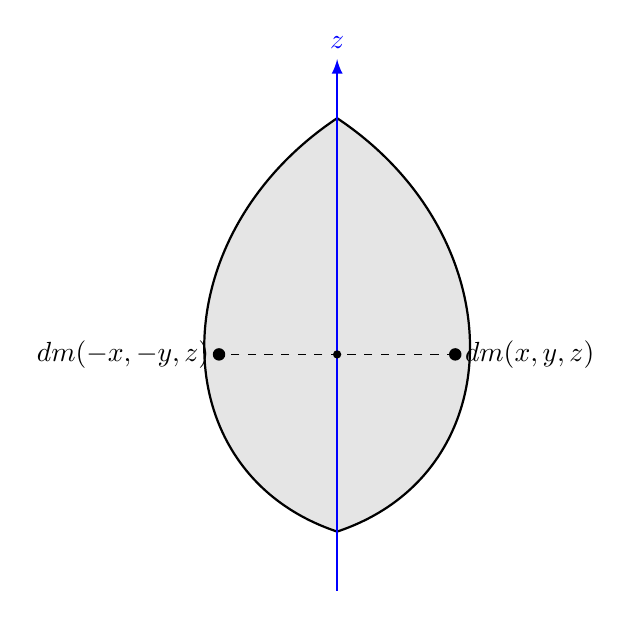
\begin{tikzpicture}[scale=1.5, >=latex]
        % Corpo simmetrico rispetto all'asse z
        \draw[thick, fill=gray!20] (0,2.5) .. controls (1.5,1.5) and (1.5,-0.5) .. (0,-1) .. controls (-1.5,-0.5) and (-1.5,1.5) .. (0,2.5);
        
        % Asse z
        \draw[->, thick, blue] (0,-1.5) -- (0,3) node[above] {$z$};
        
        % Elementi di massa simmetrici
        \coordinate (P1) at (1, 0.5);
        \coordinate (P2) at (-1, 0.5);
        
        \fill (P1) circle (1.5pt) node[right] {$dm(x,y,z)$};
        \fill (P2) circle (1.5pt) node[left] {$dm(-x,-y,z)$};
        
        % Segmento che li unisce
        \draw[dashed] (P1) -- (P2);
        \fill (0,0.5) circle (1pt);
    \end{tikzpicture}
    \caption{Corpo con asse di simmetria $z$. Ad ogni elemento di massa ad una certa distanza dall'asse corrisponde un elemento identico dalla parte opposta.}
\end{figure}
